%%%%%%%%%%%%%%%%%%%%%%%%%%%%%%%%
\section{Overview}
\label{sec:detectors-fd-ref-ov}

\begin{cdrfigure}[FD overview reference design]{FarDet-overview-SP}{Left: 3D model of the reference design for the DUNE far detector. Right: Schematic view of the detector showing the plane ordering inside the detector.}
\centering
\begin{minipage}[b]{1.0\textwidth}
\begin{center}
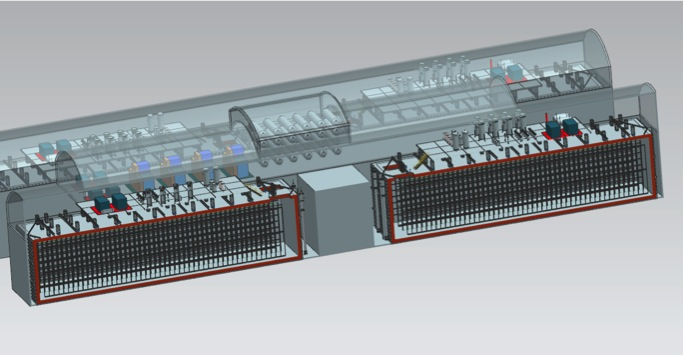
\includegraphics[width=.58\textwidth]{FarDet-3D-SP.jpg}
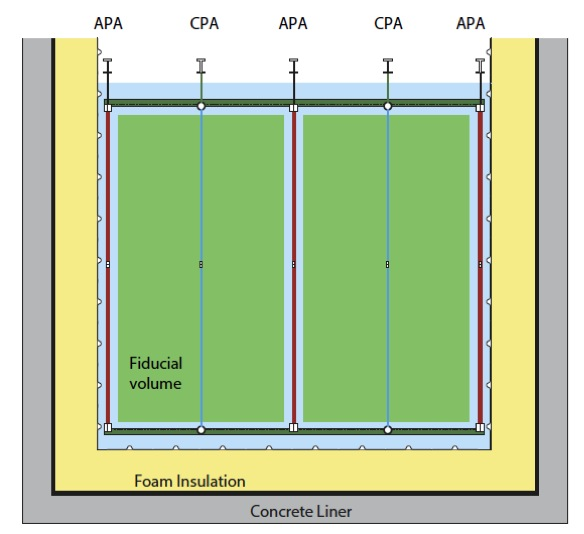
\includegraphics[width=0.38\textwidth]{FarDet-endview-SP.jpg}
\end{center}
\end{minipage}
\end{cdrfigure}

This chapter describes the reference design of the DUNE far detector. The DUNE far detector will consist of four nominal 10~kt fiducial mass liquid argon time projection chambers (TPCs) augmented with a photon detection system. It is envisioned that the detectors will be constructed in a staged fashion with the first detector coming online as soon as possible and the following detectors at a regular pace. A model of the underground experimental area with the four 10~kt detector is shown in Figure~\ref{fig:FarDet-overview-SP}. The conventional facilities planning calls for the completion of the construction of the second cryostat prior to the filling of the fist so it serves initially as a liquid storage facility. With microBooNE, the SBN experiment, and the development program through the CERN neutrino platform is expected that the detector technology will improve in the coming years. DUNE's staged program allows selection of the optimal design detector at each step. 

The reference design presented in this chapter and documented in the project cost and schedule is an array of single-phase TPCs pattered after the successful ICARUS experiment, but adapted to the local site requirements at SURF and the need to scale up the detector size. The configuration of the detector is shown on the right in Figure~\ref{fig:FarDet-overview-SP}.  The TPC detector is constructed by placing alternating high voltage cathode planes and anode readout planes in a bath of ultra-pure liquid argon (LAr). Particles interacting in the argon generate charge and VUV photons. The charge drifts in the electric field and is read out on the anode planes. A field cage around the perimeter of the anode and cathode planes insures uniform electric field in the detector volume. The DUNE far detector is  constructed from three rows of anode planes and two cathode planes running the length of the rectangular detector. The reference detector anode planes are constructed using a grid plane, two stereo wire induction planes and vertical collection plane wires. This type TPC design is referred to as a single-phase detector as the charge generation, drift, and collection are all in the liquid phase. It has the advantage that the charge is collected directly enabling precision calibration. The disadvantages are that the signal levels are low requiring the use of cold electronics and that the readout is based on stereo induction planes requiring a de-convolution of the induced signal. The TPC detector is augmented with a photon detection system to provide the t$_0$ or event time for physics processes uncorrelated with the FNAL neutrino beam.

The DUNE detector is constructed of pre-assembled and pretested anode and cathode plane modules referred to as Anode Plane Assemblies (APA) and Cathode Plane Assemblies (CPA). The size of the individual assemblies was chosen so that each assembly would fit in a HiCube shipping container, fit in the hoist at SURF, and was constructed of standard size materials. The APAs shown in Figure~\ref{fig:FarDet-overview-SP}  have an active area 2.3~m long and 6.0~m High, two APAs are hung together during installation to achieve the required 12~m tall detector. This construction has the advantage that the electronics readout can be placed at the outside of the detector minimizing the dead area in the active volume. Three APA walls each constructed of 25 double height APA cells  and two CPA walls instrument the 53~m long detector. The distance between APA and CPA is 3.6~m.


The expected performance of the DUNE far detector is based on the measure performance of the ICARUS detector, scanned Monte Carlo data, and newer studies with automated reconstruction. The projected performance is summarized in Table~\ref{tab:TPC-metric}. It is expected that as the software tools improve and both microBooNE and other dedicated test beam measurements become available the precision of the projected performance will steadily improve.


\begin{cdrtable}[DUNE Far Detector Performance Expectations]{cc}{TPC-metric}{Summary of the most important performance parameters of the DUNE reference far detector. Included are the parameters, previous detector performance, and projected performance with references to relevant studies.} 
%The third argument (reads {cc}) can use c, l, r or p{some length}  e.g. {cll} or {llp{3cm}}, for instance.
Header Column1 & Header Column 2 \\ \toprowrule
Row 1 & First \\ \colhline
Row 2 & Second \\ \colhline
Row 3 & Third \\
\end{cdrtable}


